\documentclass[tikz,border=12pt]{standalone}
\usepackage{amsmath,amssymb}
\usetikzlibrary{calc,arrows.meta,decorations.markings}

\begin{document}
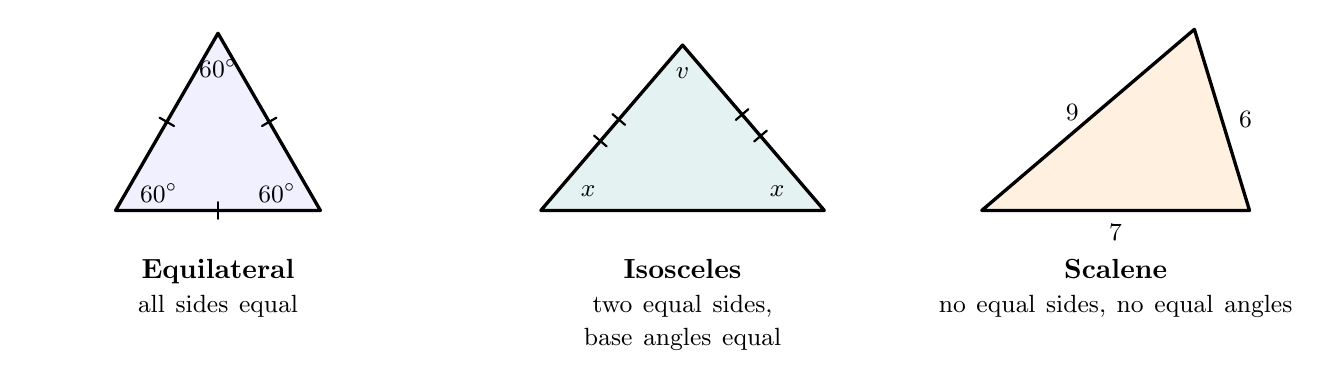
\begin{tikzpicture}[>=latex, line cap=round, line join=round]

  % ---------------- Equilateral ----------------
  \begin{scope}[shift={(0,0)}]
    \coordinate (E1) at (0,0);
    \coordinate (E2) at (2.6,0);
    \coordinate (E3) at (1.3,2.25);
    \draw[very thick, fill=blue!6] (E1)--(E2)--(E3)--cycle;
    % one tick on each side
    \draw[thick] ($(E1)!0.5!(E2)!3pt!90:(E2)$) -- ($(E1)!0.5!(E2)!3pt!270:(E2)$);
    \draw[thick] ($(E2)!0.5!(E3)!3pt!90:(E3)$) -- ($(E2)!0.5!(E3)!3pt!270:(E3)$);
    \draw[thick] ($(E3)!0.5!(E1)!3pt!90:(E1)$) -- ($(E3)!0.5!(E1)!3pt!270:(E1)$);
    \node[font=\small] at (0.55,0.22) {$60^\circ$};
    \node[font=\small] at (2.05,0.22) {$60^\circ$};
    \node[font=\small] at (1.3,1.8) {$60^\circ$};
    \node[font=\bfseries, anchor=north, align=center, text width=4.6cm] at (1.3,-0.5)
      {Equilateral\\ \normalfont\small all sides equal};
  \end{scope}

  % ---------------- Isosceles ----------------
  \begin{scope}[shift={(5.4,0)}]
    \coordinate (I1) at (0,0);
    \coordinate (I2) at (3.6,0);
    \coordinate (I3) at (1.8,2.1);
    \draw[very thick, fill=teal!10] (I1)--(I2)--(I3)--cycle;
    % double ticks on the two equal sides
    \foreach \p/\q in {I2/I3, I3/I1}{
      \draw[thick] ($(\p)!0.45!(\q)!3pt!90:(\q)$) -- ($(\p)!0.45!(\q)!3pt!270:(\q)$);
      \draw[thick] ($(\p)!0.58!(\q)!3pt!90:(\q)$) -- ($(\p)!0.58!(\q)!3pt!270:(\q)$);
    }
    \node[font=\small] at (0.6,0.25) {$x$};
    \node[font=\small] at (3.0,0.25) {$x$};
    \node[font=\small] at (1.8,1.75) {$v$};
    \node[font=\bfseries, anchor=north, align=center, text width=4.6cm] at (1.8,-0.5)
      {Isosceles\\ \normalfont\small two equal sides, base angles equal};
  \end{scope}

  % ---------------- Scalene ----------------
  \begin{scope}[shift={(11.0,0)}]
    \coordinate (S1) at (0,0);
    \coordinate (S2) at (3.4,0);
    \coordinate (S3) at (2.7,2.3);
    \draw[very thick, fill=orange!12] (S1)--(S2)--(S3)--cycle;
    \node[font=\small] at (1.7,-0.28) {$7$};
    \node[font=\small] at (3.35,1.15) {$6$};
    \node[font=\small] at (1.15,1.25) {$9$};
    \node[font=\bfseries, anchor=north, align=center, text width=4.6cm] at (1.7,-0.5)
      {Scalene\\ \normalfont\small no equal sides, no equal angles};
  \end{scope}

\end{tikzpicture}
\end{document}
